\subsection{Ansteuerung Schrittmotor}
\label{sec:stepperdriver}
Die Ansteuerung für den Schrittmotor wird in der Gruppe PREN-ET entwickelt. 
(Siehe \ref{sec:pren-et} \nameref{sec:pren-et}) 
%Daher werden hier nur Anpassungen für das Team 27 betrachtet. 
\begin{figure}[h!]
    \centering
    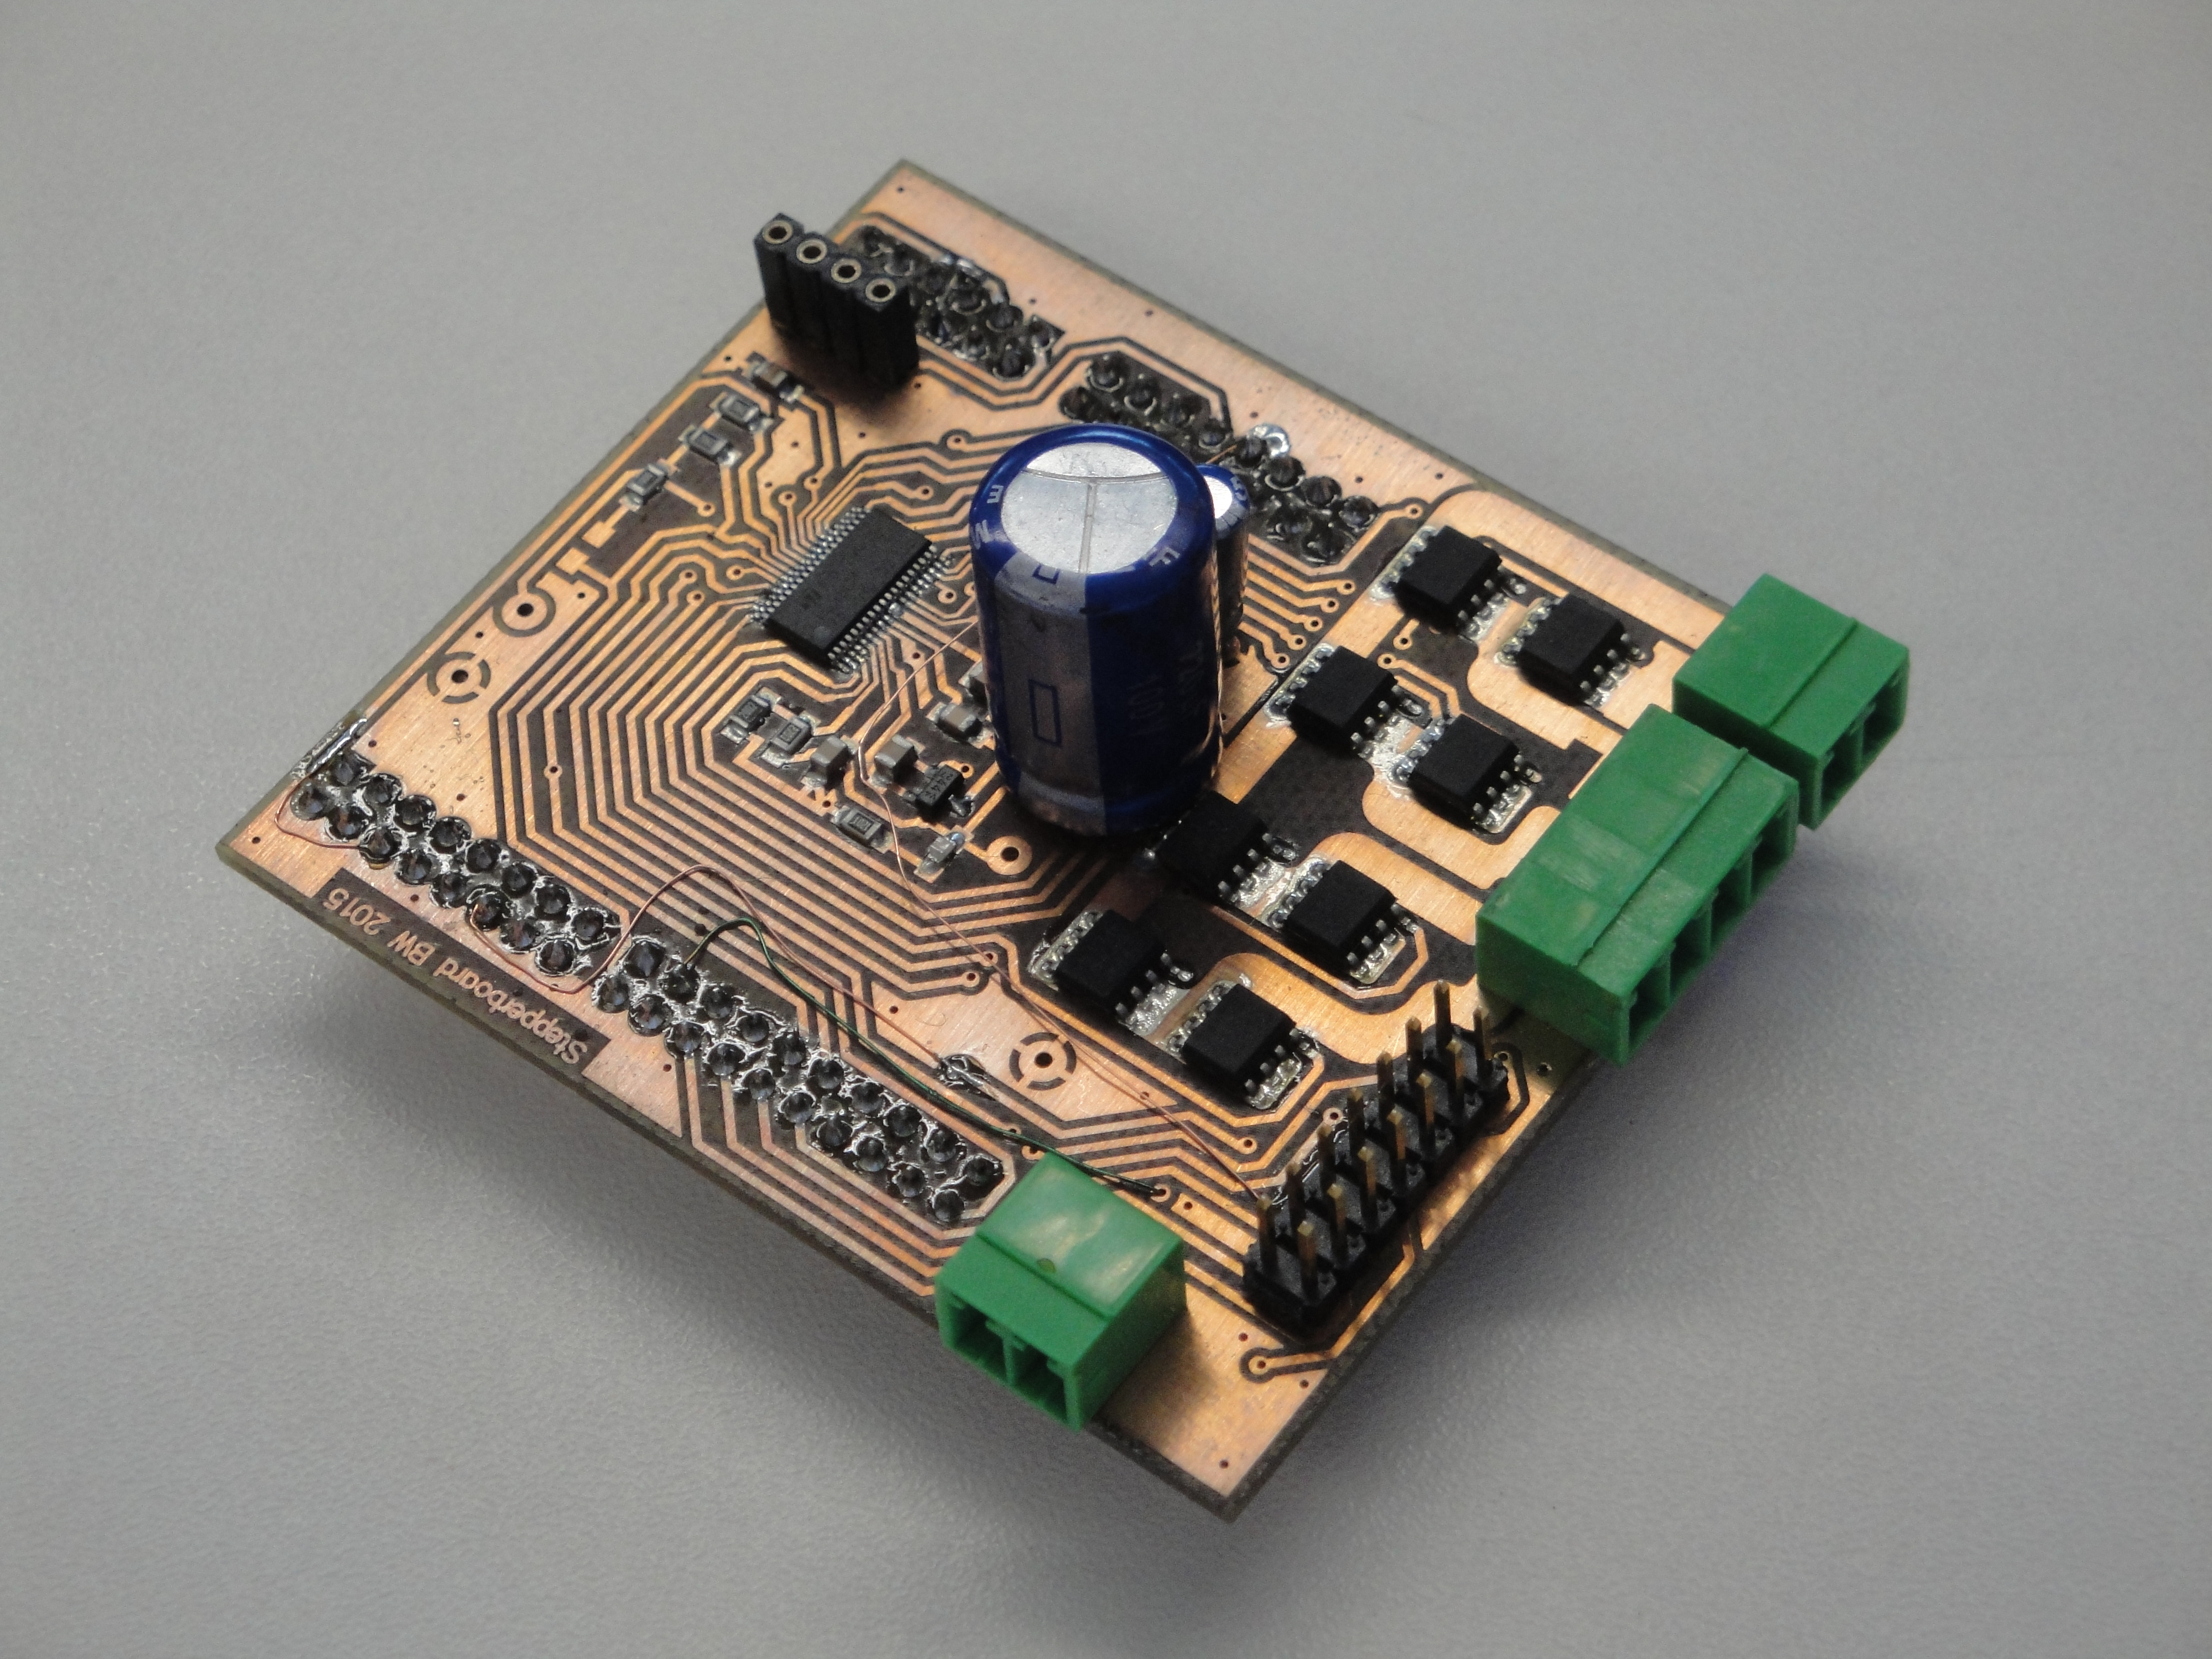
\includegraphics[width=0.7\textwidth]{fig_pcb/DSC02908.JPG}
    \caption{Ansteuerung Schrittmotor}
    \label{fig:dc}
\end{figure}

\noindent
Die Platine mit der Schrittmotoransteuerung kann direkt auf das 
Controllerboard (siehe \ref{sec:control}) gesteckt werden. Die weiteren 
Komponenten können mit einem Flachbandkabel an der Schrittmotoransteuerung 
angeschlossen werden. Das Bluetoothmodul wird direkt auf die 
Schrittmotorsteuerung gesteckt. Es kann ein bipolarer Schrittmotor 
angeschlossen werden. Dieser kann mit einer Auflösung von 1/128 Mikrosteps 
angesteuert werden. 
